%%%%%%%%%%%%%%%%%%%%%%%%%%%%%%%%%%%%%%%%%%%%%%%%%%%%%%%%%%%%%%%%%%%%%%
% How to use writeLaTeX: 
%
% You edit the source code here on the left, and the preview on the
% right shows you the result within a few seconds.
%
% Bookmark this page and share the URL with your co-authors. They can
% edit at the same time!
%
% You can upload figures, bibliographies, custom classes and
% styles using the files menu.
%
%%%%%%%%%%%%%%%%%%%%%%%%%%%%%%%%%%%%%%%%%%%%%%%%%%%%%%%%%%%%%%%%%%%%%%

\documentclass[12pt]{article}

\usepackage{sbc-template}

\usepackage{graphicx,url}

%\usepackage[brazil]{babel}   
\usepackage[utf8]{inputenc} 

\usepackage{float}
\usepackage{hyperref}
\usepackage{amsmath}

\usepackage{listings}
\usepackage{color}

\definecolor{dkgreen}{rgb}{0,0.6,0}
\definecolor{gray}{rgb}{0.5,0.5,0.5}
\definecolor{mauve}{rgb}{0.58,0,0.82}

\lstset{frame=none,
  language=C++,
  aboveskip=3mm,
  belowskip=3mm,
  showstringspaces=false,
  columns=flexible,
  basicstyle={\small\ttfamily},
  numbers=none,
  numberstyle=\tiny\color{gray},
  keywordstyle=\color{blue},
  commentstyle=\color{dkgreen},
  stringstyle=\color{mauve},
  breaklines=true,
  breakatwhitespace=true,
  tabsize=3
}

     
\sloppy

\title{Display OLED}

\author{Fabricio Araújo Dias}

\address{Instituto Federal de Educação, Ciência e Tecnologia do Ceará
  (IFCE)\\
  Avenida Vice-Presidente José Alencar, S/N -- 61.939-140 -- Maracanaú -- CE -- Brasil
  \email{fabricio.araujo61@aluno.ifce.edu.br}
}

\begin{document} 

\maketitle

\begin{abstract}
  This report details the step-by-step practical activity for the Microcontrollers course on using an display OLED SSD1306 to visualize information for the final project.
\end{abstract}
  
\begin{resumo}
  Esse relatório detalha o passo a passo da atividade prática da disciplina de Microcontroladores sobre a utilização de um display OLED SSD1306 para a visualização de informações para o projeto final.
\end{resumo}

\section{Introdução}

A décima quinta atividade prática da disciplina de Microcontroladores consistiu em utilizar um display OLED de modelo SSD1306 para exibir informações de um projeto. As equipes formadas deveriam se reunir, escolher as informações do projeto final que devem ser exibidas e experimentar.

O trabalho final de minha equipe é uma estação meteorológica doméstica que coleta como dados a temperatura do ambiente, a pressão do ar e a umidade, então desenvolvemos o código para que exiba esses dados no display toda vez que o ESP32 for iniciado, pois ele hiberna e reinicia em dada frequência.

\section{Configuração na protoboard}

Para a realização da prática, foi utilizado um ESP32 de 30 pinos, uma protoboard, um display OLED SSD1306, quatro cabos macho-fêmea e um cabo microUSB.

O display OLED ficou disposto na própria protoboard, enquanto o ESP32 ficou de fora. O display precisa de uma corrente mínima de 3.3 V para funcionar, então usamos um cabo para conectar o pino 3.3 do ESP32 ao VND do display, assim também com os pinos de GND.

Utilizamos o protocolo i2c para comunicação por ele ser bastante simples. Para isso, conferimos o pinout do ESP32 para descobrir quais pinos são próprios para a comunicação i2c, que são os pinos 21 e 22. O pino 21 é de SDA que é por onde os dados são enviados, e o pino 22 é de SCL que é o pino de clock.

\begin{figure}[H]
    \centering
    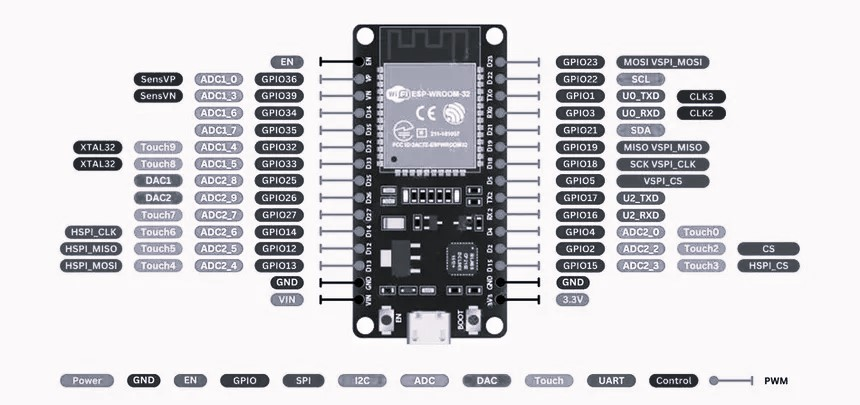
\includegraphics[width=0.5\linewidth]{img/esp32_pinout.png}
    \caption{Pinout do ESP32.}
    \label{fig:esp32-pinout}
\end{figure}

\begin{figure}[H]
    \centering
    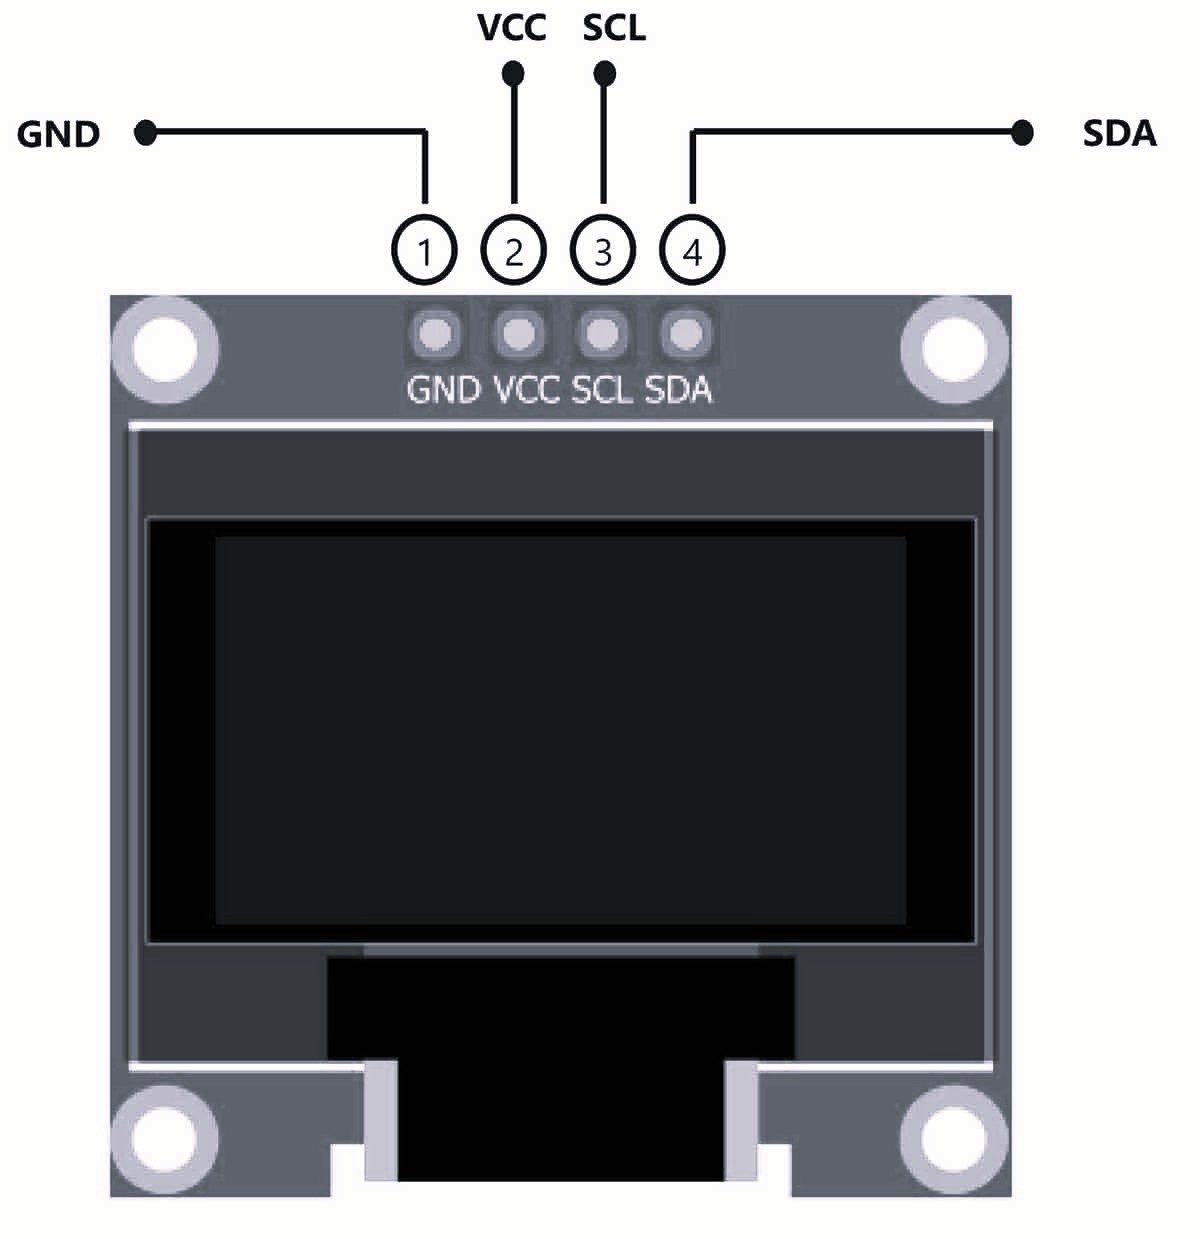
\includegraphics[width=0.5\linewidth]{img/I2C-OLED-Display-Pinout.jpg}
    \caption{Pinout do display OLED SSD1306.}
    \label{fig:enter-label}
\end{figure}

Usamos os últimos dois cabos para fazer a conexão entre os pinos de comunicação. O pino de SCL do ESP32 é conectado ao pino de SCL do display, e o mesmo é feito com o pino de SDA.

\section{Desenvolvimento do código}

Para o desenvolvimento do código, usamos o Visual Studio Code (VSCode) com a extensão do PlatformIO. Na página inicial da extensão, criamos um novo projeto com nome de "display", a placa Espressif Esp32 Dev Module e o framework Arduino.

É necessário instalar a biblioteca Adafruit SH110X. Acessamos a página de bibliotecas do PlatformIO, buscamos a biblioteca e instalamos no projeto display. No código, importamos as seguintes bibliotecas para a realização do projeto.

\begin{lstlisting}
#include <SPI.h>
#include <Wire.h>
#include <Adafruit_GFX.h>
#include <Adafruit_SH110X.h>
\end{lstlisting}

Após a instalação das bibliotecas, definimos algumas constantes no inicio do código para guardar informações sobre o display. Como o endereço MAC do display, a altura e a largura da tela em pixel. Por padrão o endereço MAC é 0x3c (pode ser 0x3d) e a resolução é 120x64. 

\begin{lstlisting}
#define i2c_Address 0x3c 
#define SCREEN_WIDTH 128 
#define SCREEN_HEIGHT 64 
\end{lstlisting}

Alguns displays podem possuir um pino extra de RESET. Como o nosso display não possui esse pino extra, informamos que o seu valor é -1. Então, instaciamos um objeto da classe Adafruit\_SH1106G e passamos a resolução, o Wire e o pino de RESET.

\begin{lstlisting}
#define OLED_RESET -1

Adafruit_SH1106G display = Adafruit_SH1106G(SCREEN_WIDTH, SCREEN_HEIGHT, &Wire, OLED_RESET);
\end{lstlisting}


Em setup, inicializamos o display com o método begin com o endereço do display e true para que o display faça hard reset se ele tiver um pino de RESET. 

\begin{lstlisting}
display.begin(i2c_Address, true);
\end{lstlisting}

Para casos onde já tenha sido escrito algo para ser mostrado no display, exibimos a mensagem e depois limpamos o buffer. Para exibir a mensagem, utilizamos o método display, e para apagar, usamos o método clearDisplay. Toda vez que usarmos o método display, é preciso definir um delay logo após para que seja possível visualizar a mensagem.

\begin{lstlisting}
display.display();

delay(2000);

display.clearDisplay();
\end{lstlisting}

Para exibir as informações que queremos, criamos uma função que é chamada no loop, pois é desejável que as informações fiquem se repetindo. 

\begin{lstlisting}
void loop() {
  drawInformations();
}
\end{lstlisting}

Em drawInformations, definimos qual é o tamanho da fonte do texto com o método setTextSize, a cor com a função setTextColor (passamos as cores que a biblioteca possui), ajustamos o cursor com a função setCursor e imprimimos mensagens com os métodos print e println. E claro, usamos display para exibir o texto e clearDisplay para limpá-lo.

\begin{lstlisting}
void drawInformations(){
  display.setTextSize(2);
  display.setTextColor(SH110X_WHITE);
  display.setCursor(0, 0);
  display.print("Temperatura: ");
  display.print("32");
  display.print((char) 247);
  display.print("C");
  display.display();
  delay(4000);
  display.clearDisplay();

  display.setTextColor(SH110X_WHITE);
  display.setCursor(0, 0);
  display.print("Umidade: ");
  display.println("72%");
  display.display();
  delay(4000);
  display.clearDisplay();

  display.setTextColor(SH110X_WHITE);
  display.setCursor(0, 0);
  display.print("Chovendo: ");
  display.println("Sim");

  display.setTextSize(1);
  display.println("Janelas fechadas");
  display.println("Varal recolhido");
  display.display();
  delay(4000);
  display.clearDisplay();
}
\end{lstlisting}

\section{Considerações finais}

\begin{figure}[H]
    \centering
    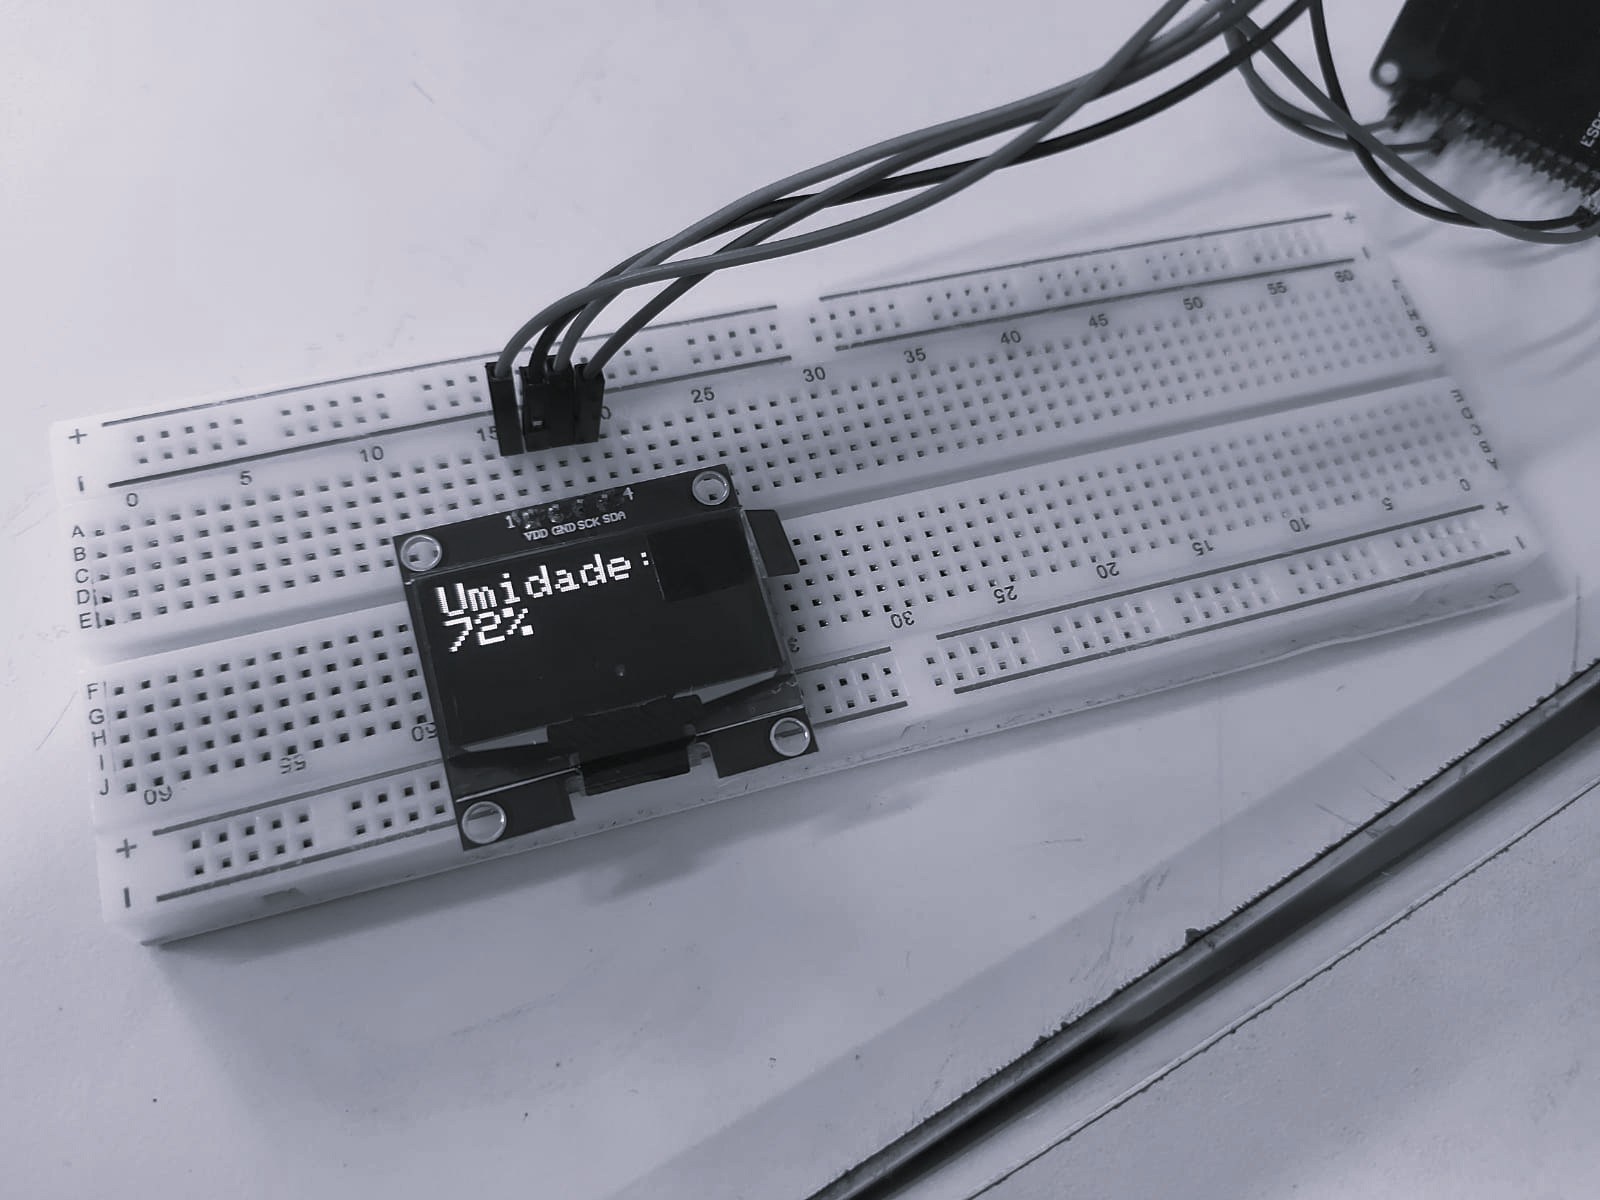
\includegraphics[width=0.5\linewidth]{img/protoboard.jpg}
    \caption{Resultado final.}
    \label{fig:protoboard}
\end{figure}

Conectado o ESP32 ao computador por meio do cabo microUSB, enviamos o código pelo atalho ALT + CTRL + U da extensão do PlatformIO. Ao terminar o envio, os dados começaram a serem exibidos na tela do display. O código pode ser conferido nesse \href{https://github.com/fabricio-araujo94/microcontroladores/tree/main/display}{repositório} no Github e o projeto em execução pode ser visto nesse \href{https://youtu.be/i_BG1nU16ck}{vídeo} no YouTube.

\end{document}